\documentclass[polish,a4paper]{article}
\usepackage{amsmath}
\usepackage{amssymb, amsfonts, amsthm, amsmath, bm}
\usepackage[T1]{fontenc}
\usepackage[utf8]{inputenc}
\usepackage{babel}
\usepackage{pslatex}
\usepackage{pgfplots}
\usepackage{hhline}
\usepackage[american]{circuitikz} 
\usepackage{anysize}
\usepackage{graphicx}
\DeclareGraphicsExtensions{.jpg}
\marginsize{2.5cm}{2.5cm}{3cm}{3cm}
\bibliographystyle{IEEEtran}


%makro do indeksów w tabeli
\newcommand{\PRzFieldDsc}[1]{\sffamily\bfseries\scriptsize #1}

%makro do informacji w tabeli
\newcommand{\PRzFieldCnt}[1]{\itshape #1}

%potężne makro tworzące tabelę z informacjami o teamie
\newcommand{\PRzHeading}[8]{
%% #1 - nazwa laboratorium
%% #2 - kierunek 
%% #3 - specjalność 
%% #4 - rok studiów 
%% #5 - symbol grupy lab.
%% #6 - temat 
%% #7 - numer lab.
%% #8 - skład grupy ćwiczeniowej

\begin{center}
\begin{tabular}{ p{0.32\textwidth} p{0.15\textwidth} p{0.15\textwidth} p{0.12\textwidth} p{0.12\textwidth} }

  &   &   &   &   \\
\hline
\multicolumn{5}{|c|}{}\\[-1ex]
\multicolumn{5}{|c|}{{\LARGE #1}}\\
\multicolumn{5}{|c|}{}\\[-1ex]

\hline
\multicolumn{1}{|l|}{\PRzFieldDsc{Kierunek}}	& \multicolumn{1}{|l|}{\PRzFieldDsc{Specjalność}}	& \multicolumn{1}{|l|}{\PRzFieldDsc{Rok studiów}}	& \multicolumn{2}{|l|}{\PRzFieldDsc{Symbol grupy lab.}} \\
\multicolumn{1}{|c|}{\PRzFieldCnt{#2}}		& \multicolumn{1}{|c|}{\PRzFieldCnt{#3}}		& \multicolumn{1}{|c|}{\PRzFieldCnt{#4}}		& \multicolumn{2}{|c|}{\PRzFieldCnt{#5}} \\

\hline
\multicolumn{4}{|l|}{\PRzFieldDsc{Temat Laboratorium}}		& \multicolumn{1}{|l|}{\PRzFieldDsc{Numer lab.}} \\
\multicolumn{4}{|c|}{\PRzFieldCnt{#6}}				& \multicolumn{1}{|c|}{\PRzFieldCnt{#7}} \\

\hline
\multicolumn{5}{|l|}{\PRzFieldDsc{Skład grupy ćwiczeniowej oraz numery indeksów}}\\
\multicolumn{5}{|c|}{\PRzFieldCnt{#8}}\\

\hline
\multicolumn{3}{|l|}{\PRzFieldDsc{Uwagi}}	& \multicolumn{2}{|l|}{\PRzFieldDsc{Ocena}} \\
\multicolumn{3}{|c|}{\PRzFieldCnt{\ }}		& \multicolumn{2}{|c|}{\PRzFieldCnt{\ }} \\

\hline
\end{tabular}
\end{center}
}
%koniec potężnego makro do tabeli

\begin{document}

%stworzenie tabeli - miejsce na zmienianie danych w tabeli
%indeksy do uzupełnienia
\PRzHeading{Laboratorium Podstaw Elektroniki}{Informatyka}{--}{I}{I1}{Diody}{4}{Ewa Fengler(132219), Sebastian Maciejewski(132275), Jan Techner(132332)}{}

%ZADANIA

\section*{Cel}
Celem przeprowadzanych doświadczeń jest zapoznanie się z układami diodowymi dzięki badaniu charakterystyki diody złączowej, konstrukcji prostownika jednopołówkowego oraz budowaniu obwodów zawierających diody świecące.

\section{Zadanie 1.2}

%1:  Zapoznaj się ze schematem (rys. 4) zestawu pomiarowego

\subsection*{2.}
Rzeczywiste wartości rezystancji wykorzystanych elementów:
%bez diody - nie jest potrzebna

\begin{center}
\begin{tabular}{|c||c|c|c|}
\hline
\textbf{Element} & \textbf{Wartość zadana} & \textbf{Oznaczenie} & \textbf{Wartość zmierzona}\\
\hhline{|=#=|=|=|}
\textbf{R1} & 1k$\Omega$ & brązowy, czarny, czerwony, złoty & $984,3\Omega\pm5\%$\\
\hline
\textbf{R2} & 3M$\Omega$ & pomarańczowy, czarny, zielony, złoty & 3,009M$\Omega\pm5\%$\\
\hline
\end{tabular}
\end{center}

%3.Przygotuj zestaw pomiarowy według rysunku 4.a

\subsection*{4.}
\begin{flushleft}
Pomiary spadków napięć $U_{R}$ na rezystorze zmierzone dla wartości napięcia źródła $U_{z}$ w zakresie $0 - 5V$ oraz obliczone wartości napięć na zaciskach diody $U_{d}$ i wartości prądów diody $I_{d}$ wyrażone jako odpowiednio:
\end{flushleft}

$$
U_{d} = U_{z} - U_{R}
$$

$$
I_{d} = \frac{U_{R}}{R}
$$

\begin{flushleft}
gdzie $R$ jest rzeczywistą (zmierzoną) wartością rezystancji opornika $R1$ wykorzystanego do konstrukcji układu.\\
Wyniki zaokrąglono do dwóch miejsc po przecinku.
\end{flushleft}

\begin{center}
\begin{tabular}{|c|c||c|c|}
\hline
\boldsymbol{$U_z$} [V] & \boldsymbol{$U_R$} [V] & \boldsymbol{$U_d$} [V]& \boldsymbol{$I_d$} [mA]\\
\hhline{|=|=#=|=|}
0 & 0 & 0 & 0\\ \hline
0,2 & 0,01 & 0,19 & 0,01\\ \hline
0,4 & 0,11 & 0,29 & 0,11\\ \hline
0,6 & 0,27 & 0,33 & 0,27\\ \hline
0,8 & 0,42 & 0,38 & 0,43\\ \hline
1 & 0,58 & 0,42 & 0,59\\ \hline
1,5 & 1,06 & 0,44 & 1,08\\ \hline
2 & 1,57 & 0,43 & 1,60\\ \hline
2,5 & 2,09 & 0,41 & 2,12\\ \hline
3 & 2,61 & 0,39 & 2,65\\ \hline
3,5 & 3,03 & 0,47 & 3,08\\ \hline
4 & 3,51 & 0,49 & 3,57\\ \hline
4,5 & 4,03 & 0,47 & 4,09\\ \hline
5 & 4,55 & 0,45 & 4,26\\ \hline
\hline
\end{tabular}
\end{center}

%5. Zmodyfikuj zestaw pomiarowy według schematu z rysunku 4.b

\subsection*{6.}
\begin{flushleft}
Podobnie jak w podpunkcie 4., w tabeli przedstawiono pomiary spadków napięć $U_{R}$ na rezystorze $R2$ (dla wyznaczonej doświadczalnie wartości jego rezystancji) zmierzone dla wartości napięcia źródła $U_{z}$ w zakresie $0 - 20V$ oraz obliczone wartości napięć na zaciskach diody $U_{d}$ i wartości prądów diody $I_{d}$ wyrażone wzorami przedstawionymi w podpunkcie 4.\\
Wyniki zaokrąglono do dwóch miejsc po przecinku, za wyjątkiem $U_{d}$, którego wartości zaokrąglono do trzech miejsc po przecinku. 

\end{flushleft}

\begin{center}
\begin{tabular}{|c|c||c|c|}
\hline
\boldsymbol{$U_z$} [V] & \boldsymbol{$U_R$} [mV] & \boldsymbol{$U_d$} [V]& \boldsymbol{$I_d$} [mA]\\
\hhline{|=|=#=|=|}
0 & 0 & 0 & 0\\ \hline
5 & 3,35 & 4,999 & 1,11\\ \hline
10 & 3,94 & 9,996 & 1,31\\ \hline
15 & 4,52 & 14,995 & 1,50\\ \hline
20 & 4,75 & 19,995 & 1,58\\ \hline
\hline
\end{tabular}
\end{center}

%7, 8. - uzupełnione tabelki: U_d = U_z - U_R, I_d = U_R/R


\subsection*{9.} [Wykres]

%Na wspólnym wykresie zobrazuj przebieg charakterystyki Id = f(Ud) dla diody spolaryzowanej w kierunku zaporowym i przewodzenia

\section{Zadanie 1.3}


\subsection*{1.} [obwód 1]
\newline

\subsection*{2.} 

\includegraphics[width=\textwidth]{50hz}

%Zaobserwuj kształt przebiegu napięcia na wejściu i wyjściu prostownika przy częstotliwości przebiegu wejściowego równej 50Hz. Zapisz oscylogram do pliku graficznego.


\subsection*{3.} Różnica amplitud napięcia między przebiegiem wejściowym oraz wyjściowym:

\begin{center}
\begin{tabular}{|l|l|}
\hline
$V_{RMS1}$ & 1,64V \\
\hline
$V_{RMS2}$ & 0,7V \\ 
\hline
różnica & 0,96V \\
\hline
\end{tabular}
\end{center}

\begin{flushleft}
Różnica między napięciami wynika z faktu, iż badany układ, jako prostownik jednopołówkowy, dokonuje częściowego wyprostowania płynącego prądu - zmienia go z prądu przemiennego na prąd tętniący, czyli prąd przemienny, z którego "usuwamy" ujemne wartości napięcia.
\end{flushleft}

%zwiększylibyście jeszcze te pola w tabeli?


\subsection*{4.} [obwód 2]


%5. Ustaw dowolnie wybraną wartość międzyszczytową napięcia Uin przebiegu wejściowego, tak aby przekraczała 2Vpp oraz dowolną częstotliwość z przedziału 50Hz...1000Hz.
%10V, 500Hz


\subsection*{6.}
% Przy pomocy multimetu zmierz wartości napięć stałych UR(DC) oraz zmiennych UR(AC) na rezystancji obciążenia R. Przy pomocy oscyloskopu wyznacz wartości międzyszczytowe napięcia UR(pp) tętnień na rezystancji R. 


\begin{center}
\begin{tabular}{|c|c||c|c|c|}
\hline
\boldsymbol{$R [\Omega]$} & \boldsymbol{$C_f [\mu F]$} & \boldsymbol{$U_{R(DC)} [V]$} & \boldsymbol{$U_{R(AC)} [V]$} & \boldsymbol{$U_{R(pp)} [V]$} \\
\hhline{|=|=#=|=|=|}
2200 & 2,2 & 3,897 & 0,436 & 1,5 \\
\hline
220	& 2,2 & 1,550 & 1,167 & 3,52 \\
\hline
220 & 20 & 2,199 & 0,236 & 0,8 \\
\hline
2200 & 20 & 3,975 & 0,050 & 0,18 \\
\hline
\end{tabular}
\end{center}

%Niby jednostki sa u gory, ale jak uznacie, ze czytelniej z jednostkami, to mozecie dopisac


\subsection*{8.} [Interpretacja] 
% Jakie zależności można dostrzec pomiędzy wielkością napięcia międzyszczytowego tętnień, wartością pojemności filtrującej Cf oraz wartością rezystancji obciążenia R?

\subsection*{9.} [Interpretacja, Teoria(?)]
% Jaka jest interpretacja pomiarów napięcia stałego (DC) oraz zmiennego (AC) w układach prostownikowych?


\section{Zadanie 1.4}


\subsection*{1.} [Obwód]
\newline

\subsection*{2.}
Wpływ wartości napięcia zasilania na świecenie diod.\\
Na zdjęciach przedstawiono świecenie diod dla napięć $5V$, $10V$ oraz $15V$.\\
\\
\textbf{1. $5V$}\\
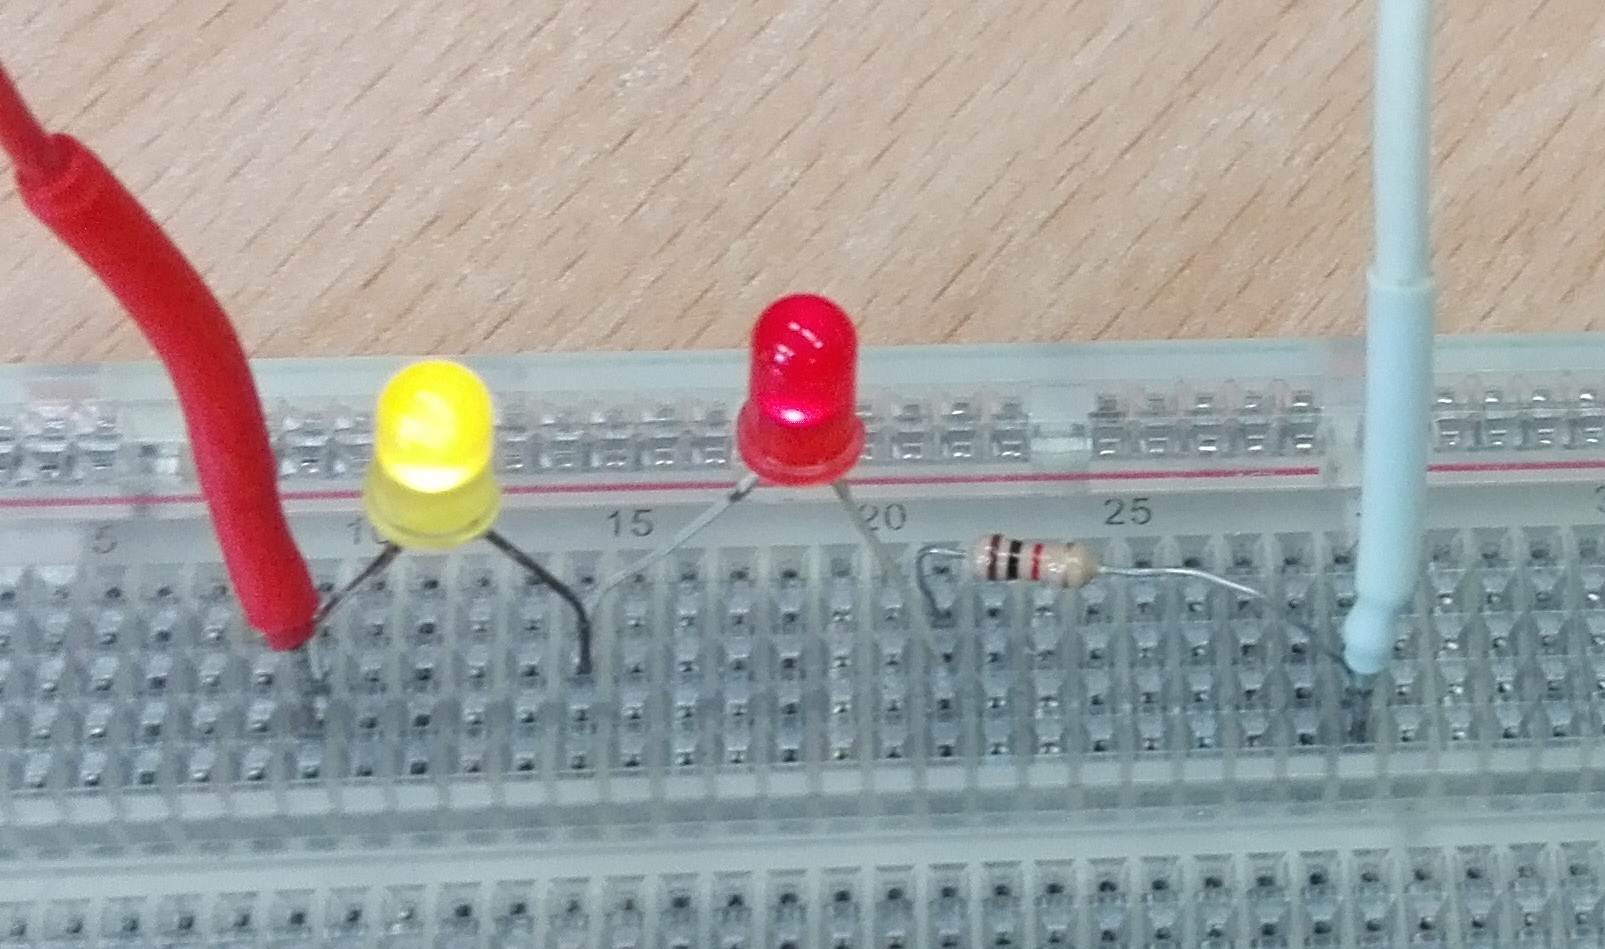
\includegraphics[width=\textwidth]{5v}
\\
\textbf{2. $10V$}\\
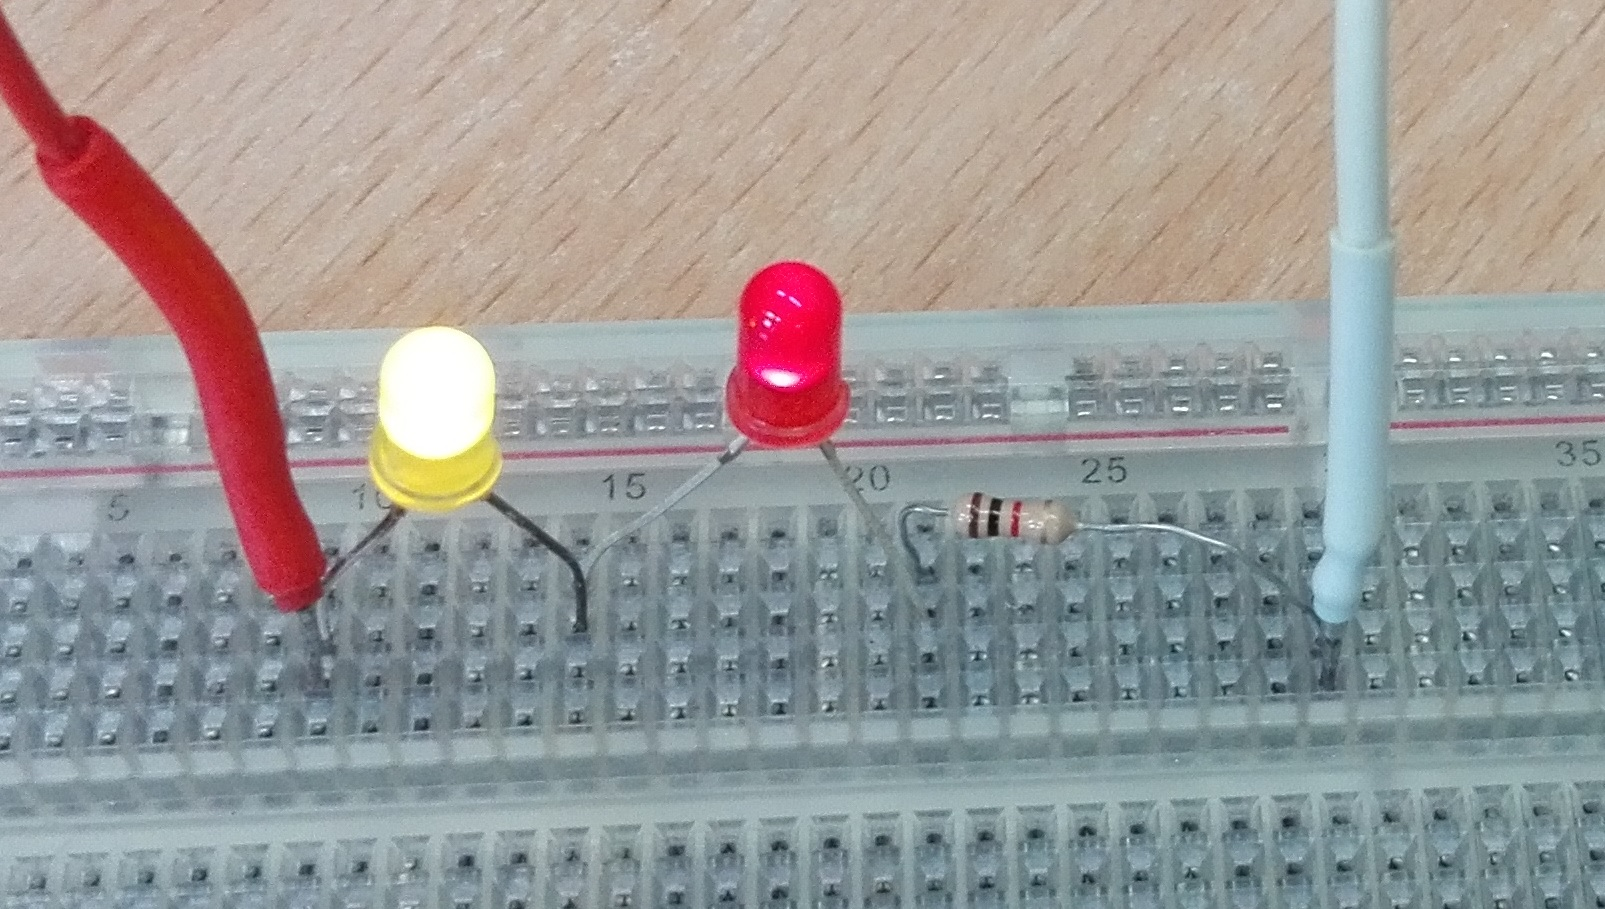
\includegraphics[width=\textwidth]{10v}
\\
\textbf{3. $15V$}\\
\includegraphics[width=\textwidth]{15V}

%Uruchom układ pomiarow. Zaobserwuj wpływ wartości napięcia zasilania na intensynowść świecenia diod.


\subsection*{3.} Spadki napięć na obu świecących diodach:
%Przy pomocy woltomierza napięcia stałego zmierz wartości spadków napięć na obu świecacych diodach. Pomiaru dokonaj z dokładnością przy najmniej 1mV .
\newline

Spadek na diodzie żółtej: 1,967V
\newline

Spadek na diodzie czerwonej: 2,036V
\newline


\subsection*{4.} [Wyjaśnienie]
%Wyjaśnij zależność między zmierzonymi spadkami napięcia a kolorem świecenia diody.

\section{Zadanie 1.5}
Cyfrą, którą mieliśmy uzyskać na wyświetlaczu była cyfra 6, poniżej przedstawiono zdjęcie i schemat połączeń niezbędnych do otrzymania takiego obrazu na wyświetlaczu.\\
\\
\textbf{Zdjęcie wyświetlacza}\\
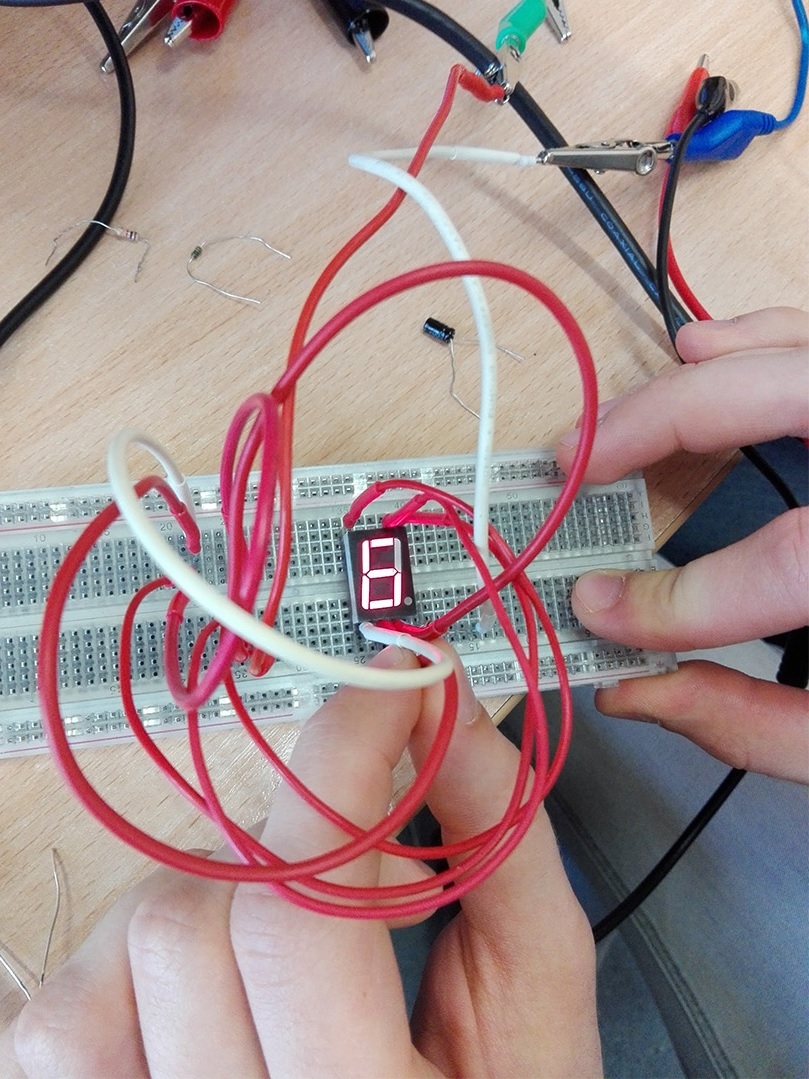
\includegraphics[width=\textwidth]{cyfra2}




[Schemat połączeń D:]


\bibliography{IEEEabrv,refs}

\begin{thebibliography}{9}

\bibitem{rlc}
  W trakcie przeprowadzania doświadczeń i pisania sprawozdania zespół korzystał głównie z materiałów ze strony http://etacar.put.poznan.pl/mariusz.naumowicz/materialy.html oraz z wiedzy własnej.

\end{thebibliography}

\end{document}7